\section{Obtención de los parámetros $q_{1}$ y $q_{2}$}

En esta sección vamos a explicar cómo obtuvimos los valores de $q_{1}$ y $q_{2}$. Éstos son parámetros que se introducen en la función \verb@hw()@ de \textit{R}. Dicha función corresponde al método Holt-Winters aditivo.

Los valores de $q_{1}$ y $q_{2}$ representan los cuantiles utilizados al calcular los intervalos de confianza. Por ejemplo, si $q_{1} = 80$ entonces se calcula el intervalo al $80\%$ de confianza. Si se introducen a la función los dos parámetros entonces se calculan dos intervalos, uno al $q_{1}\%$ de confianza y el otro al $q_{2}\%$ de confianza.

Primero definimos los parámetros generales necesarios para las simulaciones:
  
  \begin{enumerate}
\item Fijamos la semilla con \verb@set.seed(8654)@.

\item Elegimos 3 semestres para simular la demanda del número de alumnos. Los seleccionamos de los semestres que ya teníamos guardados con información real. Hicimos una comparación entre nuestros datos simulados y los reales de cada semestre. Los semestres que elegimos fueron: 2019-1, 2019-2 y 2020-1.

\item Fijamos $k = 5$ (número de semestres que se tienen como ventana de información).

\item Fijamos $num\_sim = 10$ (número de simulaciones de la demanda de alumnos para el semestre a simular).
\end{enumerate}


Después fijamos 5 materias que consideramos representativas para hacer las pruebas iniciales: \textit{Cálculo Diferencial e Integral I}, \textit{Demografía}, \textit{Modelos no Paramétricos y de Regresión}, \textit{Administración de Riesgos Financieros} y \textit{Temas Selectos de Investigación de Operaciones}.

Tomamos 12 posibles combinaciones de valores para $q_{1}$ y $q_{2}$, las cuales podemos ver en la \tablename{~\ref{valoresQ1Q2}}. La letra \textit{L} indica que se tomó la cota inferior del intervalo al $q_{1}\%$ de confianza. La letra \textit{U} indica que se tomó la cota superior del intervalo al $q_{2}\%$ de confianza.

Con estas cotas formamos intervalos de tipo $(Lq_{1}$,$Uq_{2})$. De éstos intervalos obtuvimos el número de alumnos simulados para los 3 diferentes semestres previamente definidos y para cada una de las 5 materias elegidas.

\begin{table}[H]
\centering
\begin{tabular}{|c|c|c|c|c|}
\hline 
$\textbf{q}_{\textbf{1}} \backslash \textbf{q}_{\textbf{2}}$ & \textbf{80} & \textbf{85} & \textbf{90} & \textbf{99} \\ 
\hline 
\textbf{80} & - & L80,U85 & L80,U90 & L80,U99 \\ 
\hline 
\textbf{85} & L85,U80 & - & L85,U90 & L85,U99 \\ 
\hline 
\textbf{90} & L90,U80 & L90,U85 & - & L90,U99 \\ 
\hline 
\textbf{99} & L99,U80 & L99,U85 & L99,U90 & - \\ 
\hline 
\end{tabular} 
\caption[\textit{Posibles valores para $q_{1}$ y $q_{2}$}]{\textit{Tabla que muestra todas las combinaciones de los intervalos formados con las cotas inferiores y superiores de los intervalos de confianza al $q_{1}\%$ y al $q_{2}\%$.}}\label{valoresQ1Q2}
\end{table}


Una vez hecha la simulación obtuvimos dos matrices:

\begin{enumerate}
\item Matriz de diferencias relativas: Esta matriz se genera al restar, los datos reales menos los simulados y después dividirlos entre los reales. Ésta operación se repite para cada materia y para cada simulación.

\item Matriz con información por materia: Esta matriz tiene 6 columnas: \textit{materia, intervalo, mín, media, máx} y \textit{sd}. En el renglón $i$ se tienen los datos de la matriz de diferencias relativas de la i-ésima materia para el intervalo $(Lq_{1}$,$Uq_{2})$ correspondiente. Por ejemplo, en el primer renglón de la \figurename{~\ref{matMedDispersion}} vemos que se utilizó el intervalo $(L80,U85)$ para obtener el número de alumnos simulados para el siguiente semestre de la materia \textit{Cálculo Diferencial e Integral I}. Las columnas 3 y 5 corresponden al mínimo y al máximo error relativo de la materia mencionada. Las columnas 4 y 6 indican la media y la varianza de los errores relativos de todas las simulaciones hechas para \textit{Cálculo Diferencial e Integral I}.
\end{enumerate}

\begin{figure}[H]
\centering
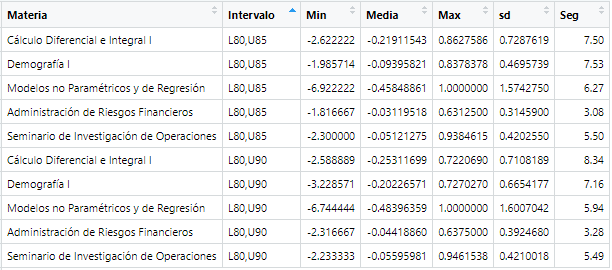
\includegraphics[width=\textwidth]{mat_med_dispersion} %scale = 0.85
\caption[\textit{Matriz con información por materia}]{\textit{Se muestran los primeros 10 renglones de la tabla obtenida con información de la matriz de diferencias relativas.}}\label{matMedDispersion}
\end{figure}


Decidimos elegir $q_{1}$ y $q_{2}$ en base a la desviación estándar. A partir de la matriz con información por materia obtuvimos una matriz de dos columnas que se muestra en la \figurename{~\ref{promSD_5m_12p}}. La nueva matriz contiene en su primer columna el intervalo $(Lq_{1}$,$Uq_{2})$ correspondiente. En la segunda el promedio de la desviación estándar para cada intervalo de las 5 materias.

\begin{figure}[H]
\centering
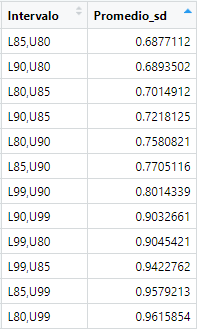
\includegraphics[scale = 1]{prom_SD_5m_12p} %width=\textwidth
\caption[\textit{Promedio de la desviación estándar: 5 materias, 12 intervalos}]{\textit{Se muestra la tabla con el promedio de la desviación estándar para 5 materias y 12 diferentes intervalos.}}\label{promSD_5m_12p}
\end{figure}


Los datos en la \figurename{~\ref{promSD_5m_12p}} están ordenados de menor a mayor con respecto al promedio de la desviación estándar. Para la segunda prueba elegimos los primeros 6 intervalos de dicha tabla y seleccionamos otras 10 materias: \textit{Álgebra Lineal I}, \textit{Álgebra Superior II}, \textit{Cómputo Evolutivo}, \textit{Análisis Matemático IV}, \textit{Matemáticas Actuariales para Seguro de Daños, Fianzas y Reaseguro}, \textit{Análisis Numérico}, \textit{Teoría de la Medida I}, \textit{Introducción a las Matemáticas Discretas}, \textit{Inglés I} y \textit{Cálculo Diferencial e Integral IV}. La tabla con el promedio de la desviación estandar de sus datos se puede ver en la \figurename{~\ref{promSD_10m_6p}}.


\begin{figure}[H]
\centering
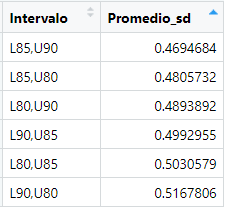
\includegraphics[scale = 1]{prom_SD_10m_6p} %width=\textwidth
\caption[\textit{Promedio de la desviación estándar: 10 materias, 6 intervalos}]{\textit{Se muestra la tabla con el promedio de la desviación estándar para 10 materias y 6 diferentes intervalos.}}\label{promSD_10m_6p}
\end{figure}


Para la tercera prueba elegimos, de la \figurename{~\ref{promSD_10m_6p}} los intervalos que tuvieran un promedio en la desviación estándar menor a $0.5$. Seleccionamos otras 10 materias: \textit{Modelos de Supervivencia y de Series de Tiempo}, \textit{Teoría del Seguro}, \textit{Programación Entera}, \textit{Investigación de Operaciones}, \textit{Geometría Moderna I}, \textit{Geometría Analítica II}, \textit{Lógica Matemática I}, \textit{Cálculo Diferencial e Integral III}, \textit{Inferencia Estadística} y \textit{Manejo de Datos}. La tabla con el promedio de la desviación estándar de sus datos se puede ver en la \figurename{~\ref{promSD_10m_4p}}.


\begin{figure}[H]
\centering
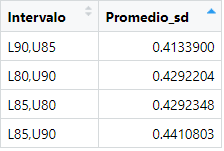
\includegraphics[scale = 1]{prom_SD_10m_4p} %width=\textwidth
\caption[\textit{Promedio de la desviación estándar: 10 materias, 4 intervalos}]{\textit{Se muestra la tabla con el promedio de la desviación estándar para 10 materias y 4 diferentes intervalos.}}\label{promSD_10m_4p}
\end{figure}

Podemos ver que los valores de la \figurename{~\ref{promSD_10m_4p}} son muy parecidos entre sí. Debido a ésto, hicimos otra prueba con los mismos intervalos pero con 5 materias obligatorias y con muchos alumnos. Las materias que elegimos fueron: \textit{Geometría Analítica I}, \textit{Cálculo Diferencial e Integral II}, \textit{Mercados Financieros y Valuación de Instrumentos}, \textit{Probabilidad II} y \textit{Procesos Estocásticos I}. Hicimos la prueba para ver si había alguna diferencia en los datos y poder elegir un solo intervalo. La tabla con el promedio de la desviación estandar de sus datos se puede ver en la \figurename{~\ref{promSD_5m_4p}}.


\begin{figure}[H]
\centering
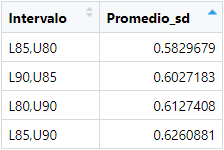
\includegraphics[scale = 1]{prom_SD_5m_4p} %width=\textwidth
\caption[\textit{Promedio de la desviación estándar: 5 materias, 4 intervalos}]{\textit{Se muestra la tabla con el promedio de la desviación estándar para 5 materias y 4 diferentes intervalos.}}\label{promSD_5m_4p}
\end{figure}

Analizando la información de las Figuras \ref{promSD_10m_4p} y \ref{promSD_5m_4p}, decidimos elegir los valores de $q_{1} = 85$ y $q_{2} = 80$. En la \figurename{~\ref{interConf}} se muestra el intervalo formado. De dicho intervalo vamos a obtener los valores para simular la demanda de alumnos para el siguiente semestre, para cada materia en cada hora.

\begin{figure}[H]
\centering
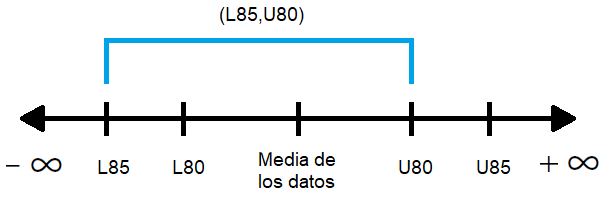
\includegraphics[scale = 0.7]{intervalos_confianza} %width=\textwidth
\caption[\textit{Diagrama de los intervalos de confianza}]{\textit{Se muestra un diagrama con el intervalo del que se va a obtener el número de alumnos para la simulación de cada materia en cada hora.}}\label{interConf}
\end{figure}

Finalmente, con los valores de $q_{1} = 85$ y $q_{2} = 80$ hicimos una prueba aleatoria (eliminando la semilla). Las materias que elegimos para dicha prueba fueron: \textit{Modelos de Supervivencia y de Series de Tiempo, Teoría del Seguro, Cálculo Diferencial e Integral I,II y III, Investigación de Operaciones, Geometría Moderna I, Geometría Analítica II, Lógica Matemática I, Probabilidad I y II, Inferencia Estadística, Manejo de Datos, Matemáticas Financieras} y \textit{Procesos Estocásticos I}. En la \figurename{~\ref{mat_med_dispersion_pruebaAl}} podemos ver los resultados de la prueba aleatoria mencionada. El promedio de la desviación estándar de todas las materias es $0.48$.%$0.4814898$.

\begin{figure}[H]
\centering
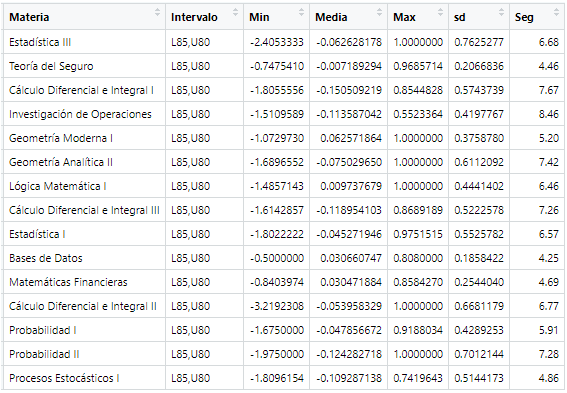
\includegraphics[width=\textwidth]{mat_med_dispersion_pruebaAleatoria} %scale = 1
\caption[\textit{Matriz con medidas de dispersión de prueba aleatoria}]{\textit{Se muestra en cada renglón la materia y el intervalo del que se tomaron los valores para la simulación. Los datos de la tabla están basados en la matriz de diferencias relativas.}}\label{mat_med_dispersion_pruebaAl}
\end{figure}
